\section{Metodologia}

A metodologia adotada para desenvolver um algoritmo de otimização consiste em definir os parâmetros de referência que buscamos atingir, desenvolver o algoritmo de otimização e aplicá-lo em cada ponto estacionário da reação buscando obter os mesmos resultados de referência.

\subsection{Parâmetros de Referência}

O artigo \cite{fh2o_first_sep} apresenta as conformações otimizadas para cada etapa da reação. Porém existe uma diferença do ponto mínimo apresentado no artigo com o obtido no módulo fortran$^{ \cite{fh2o_sep_fortran_module} }$ com interface em python, que retorna o valor de energia associado a uma determinada conformação geométrica. Dessa forma, é necessário reajustar as configurações de referência com base no módulo fortran.

% TODO: remover a citação de outras libs já que elas não foram usadas nos testes.
O processo de ajuste dos parâmetros de referência foi feito com diferentes métodos de otimização e foi escolhido o que apresentou as melhores taxas de convergência. Os métodos usados foram:
%
\begin{itemize}[itemsep=0pt,parsep=0pt]
  \item BFGS - Presente na biblioteca Scipy
  \item CG - Presente na biblioteca Scipy
  \item Newton CG - Presente na biblioteca Scipy
  \item Método de Newton
\end{itemize}
%
Dos métodos utilizados o que se apresentou mais eficaz foi o Método de Newton, que conseguiu convergir em mais casos mesmo com variações na conformação inicial.

\subsubsection{Otimização com Método de Newton}

Como apresentado na equação \eqref{eq:newton_generalization}, cada etapa de iteração é feita calculando o inverso do Jacobiano da função $G: {\mathds{R}^k\to\mathds{R}^k}, k \in \mathds{N}$. Porém no cenário de estudo dessa pesquisa temos uma função $F: {\mathds{R}^k\to\mathds{R}}, k \in \mathds{N}$, e para buscar o seu mínimo local, devemos localizar o ponto do domínio em que a norma do gradiente da função ($\nabla F$) seja zero. Dessa maneira, a etapa de iteração é calculada %TODO
%
\begin{equation}
  \mathbf{x}_{n+1} = \mathbf{x}_n - H_F(\mathbf{x}_n)^{-1} \nabla F(\mathbf{x}_n) \,,
\end{equation}
%
sendo $H_F(\mathbf{x}_n)^{-1}$ a matriz inversa $k \times k$ do Hessiano da função $F$ e $\nabla F$ o vetor gradiente da função $F$. Note que $F$ e $\mathbf{x}_n$ são, respectivamente, a função PES e as configurações da geometria da moléculas conforme descrito na seção \ref{sec:module_pes}. 

O vetor gradiente e a matriz hessiana utilizam das primeiras e segundas derivadas parciais respectivamente para serem calculadas. Por estarmos tratando de funções numéricas, não é possível obter uma expressão analítica das derivadas parciais. Nesse caso, está sendo feito o cálculo da derivada parcial numericamente utilizando a expressão
%
\begin{equation}
  \label{eq:partial_derivative}
  \frac{\partial F}{\partial x_i} \approx \frac{F(\mathbf{x}+h \mathbf{e}_i) - F(\mathbf{x}-h \mathbf{e}_i)}{2h} \,,
\end{equation}
%
onde $\mathbf{e}_i$ o iésimo vetor da base canônica de $\mathds{R}^k$ e o valor de $h = 10^{-6}$.

Dessa maneira é obtido uma média das derivadas parciais que tenderiam para direita e para a esquerda.

\subsubsection{Evitando Casos de Matriz Singular}

Esse método tem o processo de iteração interrompido caso a matriz hessiana possuir determinante igual a zero (matriz singular), que são os casos em que a matriz não possui inversa. Essa situação ocorre quando ao menos um valor do gradiente da função é zero, pois no momento de calcular a matriz hessiana haverá ao menos uma linha ou coluna com todos os valores zerados, consequentemente o determinante da matriz hessiana também será zero.

Os parâmetros dessa função descrevem a distância de ligação entre os átomos e os ângulos formados entre eles. Dependendo para qual ponto estacionário a geometria está sendo otimizada, alguns parâmetros não interferem no valor da função que retorna a energia associada a determinada configuração. Nesses casos, durante o processo de otimização é de interesse remover esses parâmetros na etapa de iteração, pois diminui a chance de se obter a matriz hessiana singular. Além disso, pelo fato de se estar calculando menos derivadas o processo de otimização fica mais rápido. 

Usando como exemplo a etapa o primeiro ponto estácionário \ce{F + H2O}, apenas 3 coordenadas são de interesse para se otimizar, como pode ser visualizado na tabela \ref{tab:relevant-var-example}.

\begin{table}[h]
\centering
  \caption{Coordenadas de interesse para otimização do ponto estacionário \ce{F + H2O}.}
\label{tab:relevant-var-example}
\resizebox{\textwidth}{!}{%
\begin{tabular}{@{}cccccccc@{}}
\toprule
  \multirow{2}{*}{Ponto Estacionário}  &  & \ce{H - O}   & \ce{O - H$'$} & \ce{H$'$-F} & \ce{HOH$'$}     & \ce{OH$'$F}     & \ce{HOH$'$F}  \\
                                       &  &  ($x_1$)     &  ($x_2$)      &  ($x_3$)    &  ($x_4$)        &  ($x_5$)        &  ($x_6$) \\ \midrule
  \ce{F + H2O} & Otimizar & \checkmark & \checkmark &  & \checkmark &  & \\ \bottomrule
\end{tabular}%
}
\end{table}

Dessa forma, reduzimos a complexidade do cálculo da matriz hessiana e do vetor gradiente, que deixa de ser calculada como 
%
\begin{equation}
  H_F =
  \begin{bmatrix}
    \frac{\partial^2 f}{\partial x_1^2} & 
    \frac{\partial^2 f}{\partial x_1 \partial x_2}& 
    \frac{\partial^2 f}{\partial x_1 \partial x_3}&  
    \frac{\partial^2 f}{\partial x_1 \partial x_4}&  
    \frac{\partial^2 f}{\partial x_1 \partial x_5}&  
    \frac{\partial^2 f}{\partial x_1 \partial x_6}\\

    \frac{\partial^2 f}{\partial x_2 \partial x_1}&
    \frac{\partial^2 f}{\partial x_2^2}&
    \frac{\partial^2 f}{\partial x_2 \partial x_3}& 
    \frac{\partial^2 f}{\partial x_2 \partial x_4}& 
    \frac{\partial^2 f}{\partial x_2 \partial x_5}& 
    \frac{\partial^2 f}{\partial x_2 \partial x_6}\\

    \frac{\partial^2 f}{\partial x_3 \partial x_1}&
    \frac{\partial^2 f}{\partial x_3 \partial x_2}&
    \frac{\partial^2 f}{\partial x_3^2}& 
    \frac{\partial^2 f}{\partial x_3 \partial x_4}&
    \frac{\partial^2 f}{\partial x_3 \partial x_5}&
    \frac{\partial^2 f}{\partial x_3 \partial x_6}\\

    \frac{\partial^2 f}{\partial x_4 \partial x_1}&
    \frac{\partial^2 f}{\partial x_4 \partial x_2}&
    \frac{\partial^2 f}{\partial x_4 \partial x_3}&
    \frac{\partial^2 f}{\partial x_4^2}&
    \frac{\partial^2 f}{\partial x_4 \partial x_5}&
    \frac{\partial^2 f}{\partial x_4 \partial x_6}\\

    \frac{\partial^2 f}{\partial x_5 \partial x_1}&
    \frac{\partial^2 f}{\partial x_5 \partial x_2}&
    \frac{\partial^2 f}{\partial x_5 \partial x_3}&
    \frac{\partial^2 f}{\partial x_5 \partial x_4}&
    \frac{\partial^2 f}{\partial x_5^2}&
    \frac{\partial^2 f}{\partial x_5 \partial x_6}\\

    \frac{\partial^2 f}{\partial x_6 \partial x_1}&
    \frac{\partial^2 f}{\partial x_6 \partial x_2}&
    \frac{\partial^2 f}{\partial x_6 \partial x_3}&
    \frac{\partial^2 f}{\partial x_6 \partial x_4}&
    \frac{\partial^2 f}{\partial x_6 \partial x_5}&
    \frac{\partial^2 f}{\partial x_6^2}\\
  \end{bmatrix}
  , \nabla F =
  \begin{bmatrix}
    \frac{\partial f}{\partial x_1}\\
    \frac{\partial f}{\partial x_2}\\
    \frac{\partial f}{\partial x_3}\\
    \frac{\partial f}{\partial x_4}\\
    \frac{\partial f}{\partial x_5}\\
    \frac{\partial f}{\partial x_6}\\
  \end{bmatrix} \,,
\end{equation}
%
passando a ser calculada
%
\begin{equation}
  H_F = 
  \begin{bmatrix}
    \frac{\partial^2 f}{\partial x_1^2}& 
    \frac{\partial^2 f}{\partial x_1 \partial x_2}&
    \frac{\partial^2 f}{\partial x_1 \partial x_4}\\

    \frac{\partial^2 f}{\partial x_2 \partial x_1}&
    \frac{\partial^2 f}{\partial x_2^2}&
    \frac{\partial^2 f}{\partial x_2 \partial x_4}\\

    \frac{\partial^2 f}{\partial x_4 \partial x_1}&
    \frac{\partial^2 f}{\partial x_4 \partial x_2}&
    \frac{\partial^2 f}{\partial x_4^2}\\
  \end{bmatrix}
  , \nabla F =
  \begin{bmatrix}
    \frac{\partial f}{\partial x_1}\\
    \frac{\partial f}{\partial x_2}\\
    \frac{\partial f}{\partial x_4}\\
  \end{bmatrix} \,.
\end{equation}
%
Aplicando o Método de Newton com base nos valores de referência dos pontos estacionários do artigo \cite{fh2o_first_sep}, foi definido as conformações a serem utilizadas como parâmetro para o presente trabalho e podem ser verificadas na tabela \ref{tab:stacionary-config}.

\begin{table}[h]
\centering
\caption{Geometrias nos Pontos Estacionários. As coordenadas relevantes referem-se as interações que mais influenciam no valor energético do ponto estacionário em estudo, essas coordenadas são as que serão otimizadas. Os valores associados as demais coordenadas são escolhidos de forma para não influenciar o processo de otimização.}
\label{tab:stacionary-config}
\resizebox{\textwidth}{!}{%
\begin{tabular}{@{}cccccccc@{}}
\toprule
  \multirow{2}{*}{Ponto Estacionário}               &                  & \ce{H - O}   & \ce{O - H$'$} & \ce{H$'$-F} & \ce{HOH$'$}    & \ce{OH$'$F}     & \ce{HOH$'$F}  \\
                                                    &                  &  ($x_1$)     &  ($x_2$)      &  ($x_3$)    &  ($x_4$)        &  ($x_5$)        &  ($x_6$) \\ \midrule
  \multirow{2}{*}{\ce{F + H2O}}                     & Vars. Relevantes & \checkmark   & \checkmark    &             & \checkmark      &                 &               \\ \cmidrule(l){2-8} 
                                                    & Valor            & 0.9609 \AA   & 0.9609 \AA    & 20 \AA      & \ang{104.1477}  & \ang{300}       & \ang{300}     \\ \midrule
  \multirow{2}{*}{\ce{R - vdW (F\bond{...}H2O)}}    & Vars. Relevantes & \checkmark   & \checkmark    & \checkmark  & \checkmark      & \checkmark      & \checkmark    \\ \cmidrule(l){2-8} 
                                                    & Valor            & 0.9641 \AA   & 0.9641 \AA    & 2.2981 \AA  & \ang{104.3416}  & \ang{67.1171}   & \ang{-87.5402} \\ \bottomrule
  \multirow{2}{*}{\ce{TS}}                          & Vars. Relevantes & \checkmark   & \checkmark    & \checkmark  & \checkmark      & \checkmark      & \checkmark    \\ \cmidrule(l){2-8} 
                                                    & Valor            & 0.9693 \AA   & 1.0250 \AA    & 1.3536 \AA  & \ang{103.2989}  & \ang{118.2898}  & \ang{68.3691}  \\ \bottomrule
  \multirow{2}{*}{\ce{P - vdW (HO\bond{...}HF)}}    & Vars. Relevantes & \checkmark   & \checkmark    & \checkmark  & \checkmark      & \checkmark      & \checkmark     \\ \cmidrule(l){2-8} 
                                                    & Valor            & 0.9728 \AA   & 1.7700 \AA    & 0.9354 \AA  & \ang{108.6504}  & \ang{173.6165}  & \ang{-0.0737} \\ \bottomrule
  \multirow{2}{*}{\ce{HO + HF}}                     & Vars. Relevantes & \checkmark   &               & \checkmark  &                 &                 &               \\ \cmidrule(l){2-8} 
                                                    & Valor            & 0.9728 \AA   & 20 \AA        & 0.9223 \AA  & \ang{300}       & \ang{300}       & \ang{300}     \\ \bottomrule
\end{tabular}%
}
\end{table}

\subsection{Funcionamento CBPB}

O método CBDP (Convergence Based in Partial Derivatives) de otimização, desenvolvido nessa pesquisa, se baseia em otimizar uma função localizando a raíz de cada uma das suas derivadas parciais individualmente. Dada uma função $F: \mathds{R}^k \to \mathds{R}, k \in \mathds{N}$ o método busca identificar o ponto em que o módulo do valor máximo das deriviadas parciais seja menor que um valor de tolerância, sendo um valor próximo de zero
%
\begin{equation}
  \label{eq:convergence-criteria}
  \max_{i \in \{1,...,k\} } \Bigg| \frac{ \partial F}{\partial x_i} \Bigg| < \text{tolerance} \approx 0 \,.
\end{equation}
%
Nesse método, cada etapa da iteração é calculada
%
\begin{equation}
  \mathbf{x}_{n+1} = \mathbf{x}_n - \diag{\left(\frac{\partial^2 F}{\partial (x_{n})^2 }\right)}^{-1} \nabla F(\mathbf{x}_n) \,,
\end{equation}
%
sendo diag a matriz diagonal da matriz hessiana da função $F$. Cada coordenada $(x_{n+1})_i$ do vetor $\mathbf{x}_{n+1}$ pode ser calculada
%
\begin{equation}
  (x_{n+1})_i = (x_{n})_i - \left( \frac{\partial^2 F}{\partial (x_{n})_i^2 } \right)^{-1} \frac{\partial F}{\partial (x_{n})_i} , i \in \{1,...,k\} \,,
\end{equation}
%
em que utilizando da notação definida em \eqref{eq:partial_derivative} definimos
%
\begin{equation}
  \label{eq:partial-derivative-aprox}
  \begin{split}
    \frac{\partial F}{\partial (x_{n})_i}      & \approx \frac{F(\mathbf{x}_n + h \mathbf{e}_i) - F(\mathbf{x}_n - h \mathbf{e}_i)}{2h} \\
    \frac{\partial^2 F}{\partial (x_{n})_i^2 } & \approx \frac{\frac{\partial F(\mathbf{x}_n + h \mathbf{e}_i) }{\partial (x_{n})_i } - \frac{\partial F(\mathbf{x}_n - h \mathbf{e}_i)}{\partial (x_{n})_i }}{2h} \,.
  \end{split}
\end{equation}


\subsubsection{Interpretação do Método}

O método se baseia em olhar para o problema de otimização tratando cada variável da função a ser otimizada de maneira independente. Tomamos cada derivada parcial $\frac{\partial F}{\partial x_i}$ da função $F \in \mathds{R}^k$ e aplicamos o Método de Newton (\ref{sec:newton-method}) em cada uma dessas derivadas parcias, usando as aproximações para a primeira e segunda derivada parcial definidas em (\ref{eq:partial-derivative-aprox}).

Tomamos como exemplo a função $F(x,y) = 1.5x^2 + 1.2y^2 - 0.25x^4 - 0.3y^4$ com o ponto inicial $\mathbf{P}_0 = (x_0,y_0) = (1, 0.8)$ que possui como derivadas parciais
%
\begin{equation}
  \begin{split}
    \frac{\partial F}{\partial x} = 3x - x^3 \\
    \frac{\partial F}{\partial y} = 2.4y - 1.2y^3 \,.
  \end{split}
\end{equation} 
%
Uma etapa de iteração para calcular o ponto $\mathbf{P}_1 = (x_1,y_1)$ é feito calculando
\begin{equation}
  \begin{split}
    x_1 = x_0 - \frac{1}{3x_0 - x_0^3} F(x_0, y_0) = 0.05\\
    y_1 = y_0 - \frac{1}{2.4y_0 - 1.2y_0^3} F(x_0, y_0) \approx -0.65 \,,
  \end{split}
\end{equation}
%
definindo $\mathbf{P}_1 = (x_1,y_1) = (0.05, -0.65)$. Geometricamente esse processo é interpretado como na figura \ref{fig:cbpd_geom_interp}.

\begin{figure}
  \begin{center}
    \pgfplotsset{compat=newest}
\pgfplotsset{
  layers/my layer set/.define layer set={
    background,
    main,
    foreground
  }{},
  set layers=my layer set,
}

\begin{center}
  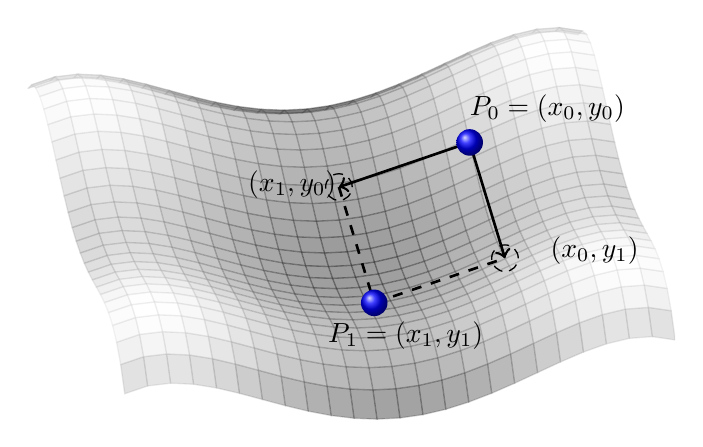
\begin{tikzpicture}[
      scale = 1.2
    ]
    \begin{axis}[
        view={-10}{60},
        zmin=-2,
        zmax=5,
        colormap/blackwhite,
        hide axis,
        xlabel=$x$,
        ylabel=$y$,
        z buffer=sort
      ]


      \addplot3 [
          surf,
          shader=faceted,
          opacity=0.2,
          fill opacity=0.4,
          samples=25,
          domain=-2:2,
          y domain=-2:2,
        ] {1.5*x^2 + 1.2*y^2 - 0.25*x^4 - 0.3*y^4};
      
      \addplot3 [
        draw=none, 
        mark=ball, 
        mark size=4, 
        z
      ] table[row sep=crcr] {%
          1     0.8     1.895\\
          0.05  -0.655  0.463 \\
        };
      
      \addplot3 [
        draw = none, 
        mark = o, 
        mark size=4,
        mark options = {
          densely dashed
        },
        z
      ] table[row sep=crcr] {%
          0.05  0.8   0.649 \\
          1     -0.655   1.710 \\
        };
      
      \addplot3 [
        <-, 
        thick, 
        black,
        z
      ] coordinates {
        (1,0.8,1.895) 
        (0.05,0.8, 0.649)
      };
      
      \addplot3 [
        -, 
        thick, 
        black,
        dashed,
        z
      ] coordinates {
        (0.05,0.8, 0.649)
        (0.05,-0.655, 0.463)
      };
      
      \addplot3 [
        ->, 
        thick, 
        black,
        z
      ] coordinates {
        (1,0.8,1.895) 
        (1,-0.655, 1.710)
      };
      
      \addplot3 [
        -, 
        thick, 
        black,
        dashed,
        z
      ] coordinates {
        (1,-0.655, 1.710)
        (0.05,-0.655, 0.463)
      };

      % \node[font=\bfseries, above] at (axis cs: 1.2, 0.8, 1.895) {$P_0 = (x_0, y_0)$};
      % \node[font=\bfseries, below] at (axis cs: 0.05, -0.655, 0.463) {$P_1 = (x_1, y_1)$};
    \end{axis}

    % \draw[step=1cm,gray,very thin] (0,0) grid (12,8);
    
    \node[font=\bfseries] at (5.5,4.1) {$P_0 = (x_0, y_0)$};
    \node[font=\bfseries] at (4,1.7) {$P_1 = (x_1, y_1)$};
    
    \node[font=\bfseries] at (6,2.6) {$(x_0, y_1)$};
    \node[font=\bfseries] at (2.8,3.3) {$(x_1, y_0)$};

  \end{tikzpicture}
\end{center}


  \end{center}
  \caption{Representação geométrica de uma etapa do método de convergência CBPD.}
  \label{fig:cbpd_geom_interp}
\end{figure}

O procedimento é repetido até atingir o critério de convergência (\ref{eq:convergence-criteria}) ou até atingir um valor máximo arbitrário de iterações.


\subsection{Avaliando Eficiência do Algoritmo}

\subsubsection{Variando uma Coordenada}

A primeira estratégia que será utilizada é, para cada ponto estacionário, como que o algoritmo se comporta quando apenas uma coordenada se distância da conformação ideal. Nessa abordagem todas as coordendas ficam em seu valor ótimo com exceção da coordenda que está variando. Dessa maneira estaremos trabalhando com um problema em apenas uma dimensão.

Para cada ponto estacionário da reação será analisado uma coordenada relevante de cada vez, variando ela em \textit{-25\%, -20\%, -15\%, 10\%, -5\%, 0\%, 5\%, 10\%, 15\%, 20\%, 25\%} do seu valor otimizado.

Exemplificando para o caso \ce{F + H2O} haverão 11 cenários de tentativa de convergência para a primeira coordenada (Ligação \ce{H + O}) como apresentados na tabela \ref{tab:conv_one_var}. O mesmo processo será feito para todas as demais coordenadas relevantes.

\begin{table}[h]
  \centering
    \caption{Cenários de convergência do método de variação de uma coordenada para a coordenada \ce{H-O} do ponto estacionário \ce{F + H2O}}
    \label{tab:conv_one_var}
    \begin{adjustbox}{width=0.6\textwidth}
    \begin{tabular}{@{}ccccccc@{}}
      \toprule
      \multirow{2}{*}{Caso} &  \ce{H - O} & \ce{O - H$'$} & \ce{H$'$-F}  & \ce{HOH$'$}     & \ce{OH$'$F}     & \ce{HOH$'$F}  \\
          & ($x_1$) & ($x_2$) & ($x_3$) & ($x_4$) &  ($x_5$)  &  ($x_6$) \\ \midrule
      1   & 0.7207 \AA & 0.9609 \AA & 20 \AA & \ang{104.1477} & \ang{300} & \ang{300} \\ \midrule
      2   & 0.7687 \AA & 0.9609 \AA & 20 \AA & \ang{104.1477} & \ang{300} & \ang{300} \\ \midrule
      3   & 0.8168 \AA & 0.9609 \AA & 20 \AA & \ang{104.1477} & \ang{300} & \ang{300} \\ \midrule
      4   & 0.8648 \AA & 0.9609 \AA & 20 \AA & \ang{104.1477} & \ang{300} & \ang{300} \\ \midrule
      5   & 0.9128 \AA & 0.9609 \AA & 20 \AA & \ang{104.1477} & \ang{300} & \ang{300} \\ \midrule
      6   & 0.9609 \AA & 0.9609 \AA & 20 \AA & \ang{104.1477} & \ang{300} & \ang{300} \\ \midrule
      7   & 1.0089 \AA & 0.9609 \AA & 20 \AA & \ang{104.1477} & \ang{300} & \ang{300} \\ \midrule
      8   & 1.0570 \AA & 0.9609 \AA & 20 \AA & \ang{104.1477} & \ang{300} & \ang{300} \\ \midrule
      9   & 1.1050 \AA & 0.9609 \AA & 20 \AA & \ang{104.1477} & \ang{300} & \ang{300} \\ \midrule
      10  & 1.1531 \AA & 0.9609 \AA & 20 \AA & \ang{104.1477} & \ang{300} & \ang{300} \\ \midrule
      11  & 1.2011 \AA & 0.9609 \AA & 20 \AA & \ang{104.1477} & \ang{300} & \ang{300} \\ \bottomrule
    \end{tabular}%
    \end{adjustbox}
\end{table}

\subsubsection{Cenários Aleatórios de Convergência}

A segunda métrica que será utilizada busca explorar a convergência quando múltiplas coordenadas não estão em sua configuração ótima. Para isso, para cada etapa da reação química que possui a sua configuração otimizada, serão geradas 100 configurações distorciadas, nas quais a variação máxima para as ligações serão de $\pm 0.3$ \AA{} e para ângulos serão de $\pm \ang{10}$. Os valores mínimos e máximos para cada estado estácionário podem ser verificados na tabela \ref{tab:min-max-config-values}.

\begin{table}[h]
\centering
  \caption{Valores mínimos e máximos que podem ser gerados nos cenários aleatórios de convergência para cada ponto estacionário da reação \ce{F + H2O -> FH + HO}}
  \label{tab:min-max-config-values}
\resizebox{\textwidth}{!}{%
\begin{tabular}{@{}cccccccc@{}}
\toprule
  \multirow{2}{*}{Ponto Estacionário}               &            & \ce{H - O}   & \ce{O - H$'$} & \ce{H$'$-F} & \ce{HOH$'$}     & \ce{OH$'$F}     & \ce{HOH$'$F}  \\
                                                    &            &  ($x_1$)     &  ($x_2$)      &  ($x_3$)    &  ($x_4$)        &  ($x_5$)        &  ($x_6$) \\ \midrule
  \multirow{2}{*}{\ce{F + H2O}}                     & Valor Mín. & 0.6609 \AA   & 0.6609 \AA    & 19.7 \AA    & \ang{94.1477}  & \ang{290}  & \ang{290} \\ \cmidrule(l){2-8} 
                                                    & Valor Máx. & 1.2609 \AA   & 1.2609 \AA    & 20.3 \AA    & \ang{114.1477}  & \ang{310}  & \ang{310} \\ \midrule
  \multirow{2}{*}{\ce{R - vdW (F\bond{...}H2O)}}    & Valor Mín. & 0.6641 \AA   & 0.6641 \AA    & 1.9981 \AA  & \ang{94.3416}  & \ang{57.1171}  & \ang{-97.5402} \\ \cmidrule(l){2-8} 
                                                    & Valor Máx. & 1.2641 \AA   & 1.2641 \AA    & 2.5981 \AA  & \ang{114.3416}  & \ang{77.1171}  & \ang{-77.5402} \\ \bottomrule
  \multirow{2}{*}{\ce{TS}}                          & Valor Mín. & 0.6693 \AA   & 0.7270 \AA    & 1.0536 \AA  & \ang{93.2989}  & \ang{108.2898}  & \ang{58.3691} \\ \cmidrule(l){2-8} 
                                                    & Valor Máx. & 1.2693 \AA   & 1.3250 \AA    & 1.6536 \AA  & \ang{113.2989}  & \ang{128.2898}  & \ang{78.3691} \\ \bottomrule
  \multirow{2}{*}{\ce{P - vdW (HO\bond{...}HF)}}    & Valor Mín. & 0.6728 \AA   & 1.4700 \AA    & 0.6354 \AA  & \ang{98.6504}  & \ang{163.6165}  & \ang{-10.0737} \\ \cmidrule(l){2-8} 
                                                    & Valor Máx. & 1.2728 \AA   & 2.0700 \AA    & 1.2354 \AA  & \ang{118.6504}  & \ang{183.6165}  & \ang{9.9263} \\ \bottomrule
  \multirow{2}{*}{\ce{HO + HF}}                     & Valor Mín. & 0.6728 \AA   & 19.7 \AA      & 0.6223 \AA  & \ang{290}  & \ang{290}  & \ang{290} \\ \cmidrule(l){2-8} 
                                                    & Valor Máx. & 1.2728 \AA   & 20.3 \AA      & 1.2223 \AA  & \ang{310}  & \ang{310}  & \ang{310} \\ \bottomrule
\end{tabular}%
}
\end{table}
